\documentclass[conference]{IEEEtran}
\IEEEoverridecommandlockouts
\usepackage{cite}
\usepackage{amsmath,amssymb,amsfonts}
\usepackage{algorithmic}
\usepackage{graphicx}
\usepackage{textcomp}
\usepackage{xcolor}
\def\BibTeX{{\rm B\kern-.05em{\sc i\kern-.025em b}\kern-.08em
    T\kern-.1667em\lower.7ex\hbox{E}\kern-.125emX}}
\begin{document}

\title{
SONAR with HC-SR04 and Object Classification with ESP32-CAM\\
\thanks
}

\author{\IEEEauthorblockN{1\textsuperscript{st} Farid Anfasha}
\IEEEauthorblockA{\textit{Informatics} \\
\textit{Insitut Teknologi Sumatera}\\
South Lampung, Indonesia \\
farid.119140215@student.itera.ac.id}
\and
\IEEEauthorblockN{2\textsuperscript{nd} Andhika Putra Pratama}
\IEEEauthorblockA{\textit{Informatics} \\
\textit{Insitut Teknologi Sumatera}\\
South Lampung, Indonesia \\
andhika.119140224@student.itera.ac.id}
\and
\IEEEauthorblockN{3\textsuperscript{rd} Rayhan Athalla Ghifary}
\IEEEauthorblockA{\textit{Informatics} \\
\textit{Insitut Teknologi Sumatera}\\
South Lampung, Indonesia \\
rayhan.1191402255@student.itera.ac.id}
}

\maketitle

\begin{abstract}
SONAR (Sound Navigation And Ranging) is a system that detects an object by sending a sound signal and waiting for an echo to detect a target. The type of SONAR signal used to detect the target position is pulse wave. The transducer used is the HC-SR04 sensor. There is also an additional Embedded Vision to view and classify objects automatically using COCO-SSD. COCO-SSD (SSD stands for Single Shot Detection) is a model for classifying objects according to the COCO dataset. In this final project, we combine COCO-SSD with HC-SR04 so that it can classify objects and see the distance between objects and sensors.
\end{abstract}

\begin{IEEEkeywords}
Classification, COCO-SSD, Ultrasonic, Vision
\end{IEEEkeywords}

% BAB 1
\section{Introduction}
In the process of observing or seeing visual limitations in detecting an object is called limited visibility, the cause can be caused by various things, one of which is poor lighting conditions, technology promises a solution in overcoming the limited visibility \cite{b1}. One technology that can detect and calculate the distance of objects is SONAR.

SONAR (Sound Navigation And Ranging) is a remote object detection system by captures the reflected signal emitted \cite{b2}. In the world of biology, sonar systems can be found in bats and dolphins. Sonar utilizes sound waves to detect very high (ultrasonic) to very low (infrasonic) frequencies \cite{b2}.

Ultrasonic sensors work by emitting ultrasonic waves originating from the transmitter in the form of a special frequency and within a certain duration, where the value of the emitted frequency is above 20kHz, then after the signal is emitted the signal will hit the object in front of it and then reflected to the object. transmitter (sender), here the transmitter also acts as a receiver (receiver), based on the reflection, the process of calculating the object distance will be carried out with the formula Distance Object = Wave Speed x Time / 2 \cite{b3}.

Based on the description that has been explained, the ultrasonic sensor can be useful for detecting objects in an area. By using an ultrasonic sensor driven by a motor, we can design an object detection system with the concept of SONAR up to a 180-degree rotation angle and the use of a camera can add SONAR functions to be able to see and recognize objects in real-time if an object is detected by the ultrasonic sensor HC-SR04.

%BAB 2
\section{Study Literature}
\subsection{Arduino IDE}
Arduino IDE is an application which functions or is used as a program developer and can upload the program to the Arduino board or ESP32\cite{b4}.
\subsection{COCO-SSD}
This model is a TensorFlow.js port of the COCO-SSD model. This model detects objects based on large-scale COCO datasets. The model can detect 80 classes of objects such as cat, dog, person, doll, bottle, tv, laptop, and etc. While SSD (SSD stands for Single Shot MultiBox Detection) is an algorithm used to detect and classify objects in this model\cite{b5}.
\subsection{ESP32-Dev-Kit}
The ESP32 microcontroller is the successor of the ESP8266 Microcontroller which is also known as the Espressif System of the ESP8266 Microcontroller. The ESP32 microcontroller chip already supports the use of a WiFi module so that it can create an IoT (Internet of Things)-based application system\cite{b6}.
\subsection{ESP32-CAM}
The ESP32-CAM module is a tool that can take data or sensors in the form of images by working like a motion detection camera. ESP32-CAM also includes a complete module that has a microcontroller and also ESP32-CAM can function as a WIFI module to transmit images to the target device\cite{b7}.

%BAB 3
\section{Architecture}
\subsection{Software}
In this final project, the software used is Arduino IDE which has added an ESP32 board and an ESP32 Servo library. The model used for object classification is one part of Tensorflow.js, namely COCO-SSD.

\subsection{Hardware}
The components that we use for this final project are ESP32 Dev Kit, ESP32-CAM, FTDI FT232RL, Ultrasonic HC-SR04, Dual Axis Joystick Module, Micro Servo MG90S, Buzzer, Push Button, Jumper, XY Bracket, and Breadboard.

\subsection{System Architecture}
The system architecture that we designed can be seen in the image below:
\begin{figure}[htbp]
\centerline{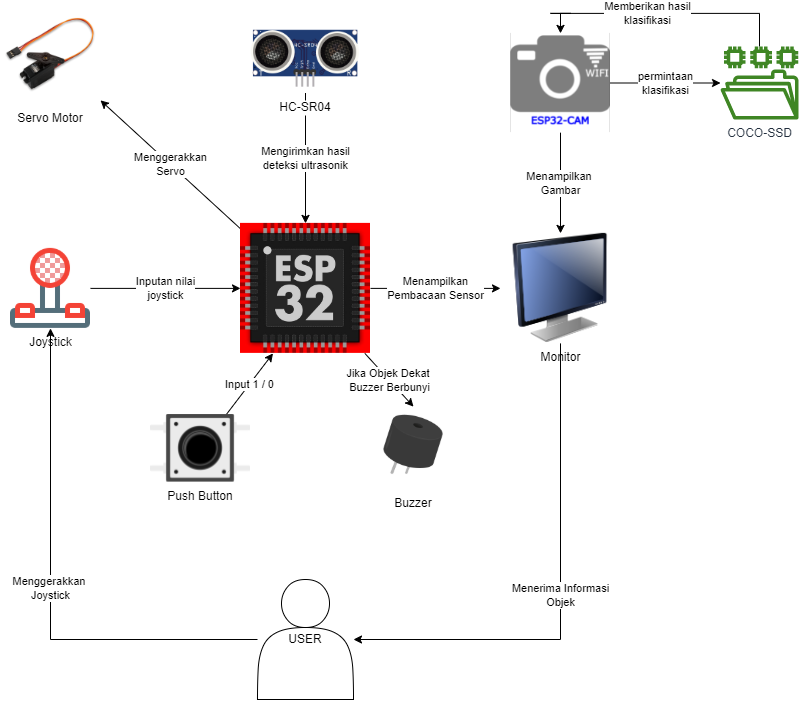
\includegraphics[width=8cm, height=8cm]{Lampiran/sysarch.png}}
\caption{System Architecture}
\label{sysarch}
\end{figure}

\subsection{Wiring Diagram}
The wiring diagram that we designed can be seen in the image below:
\begin{figure}[htbp]
\centerline{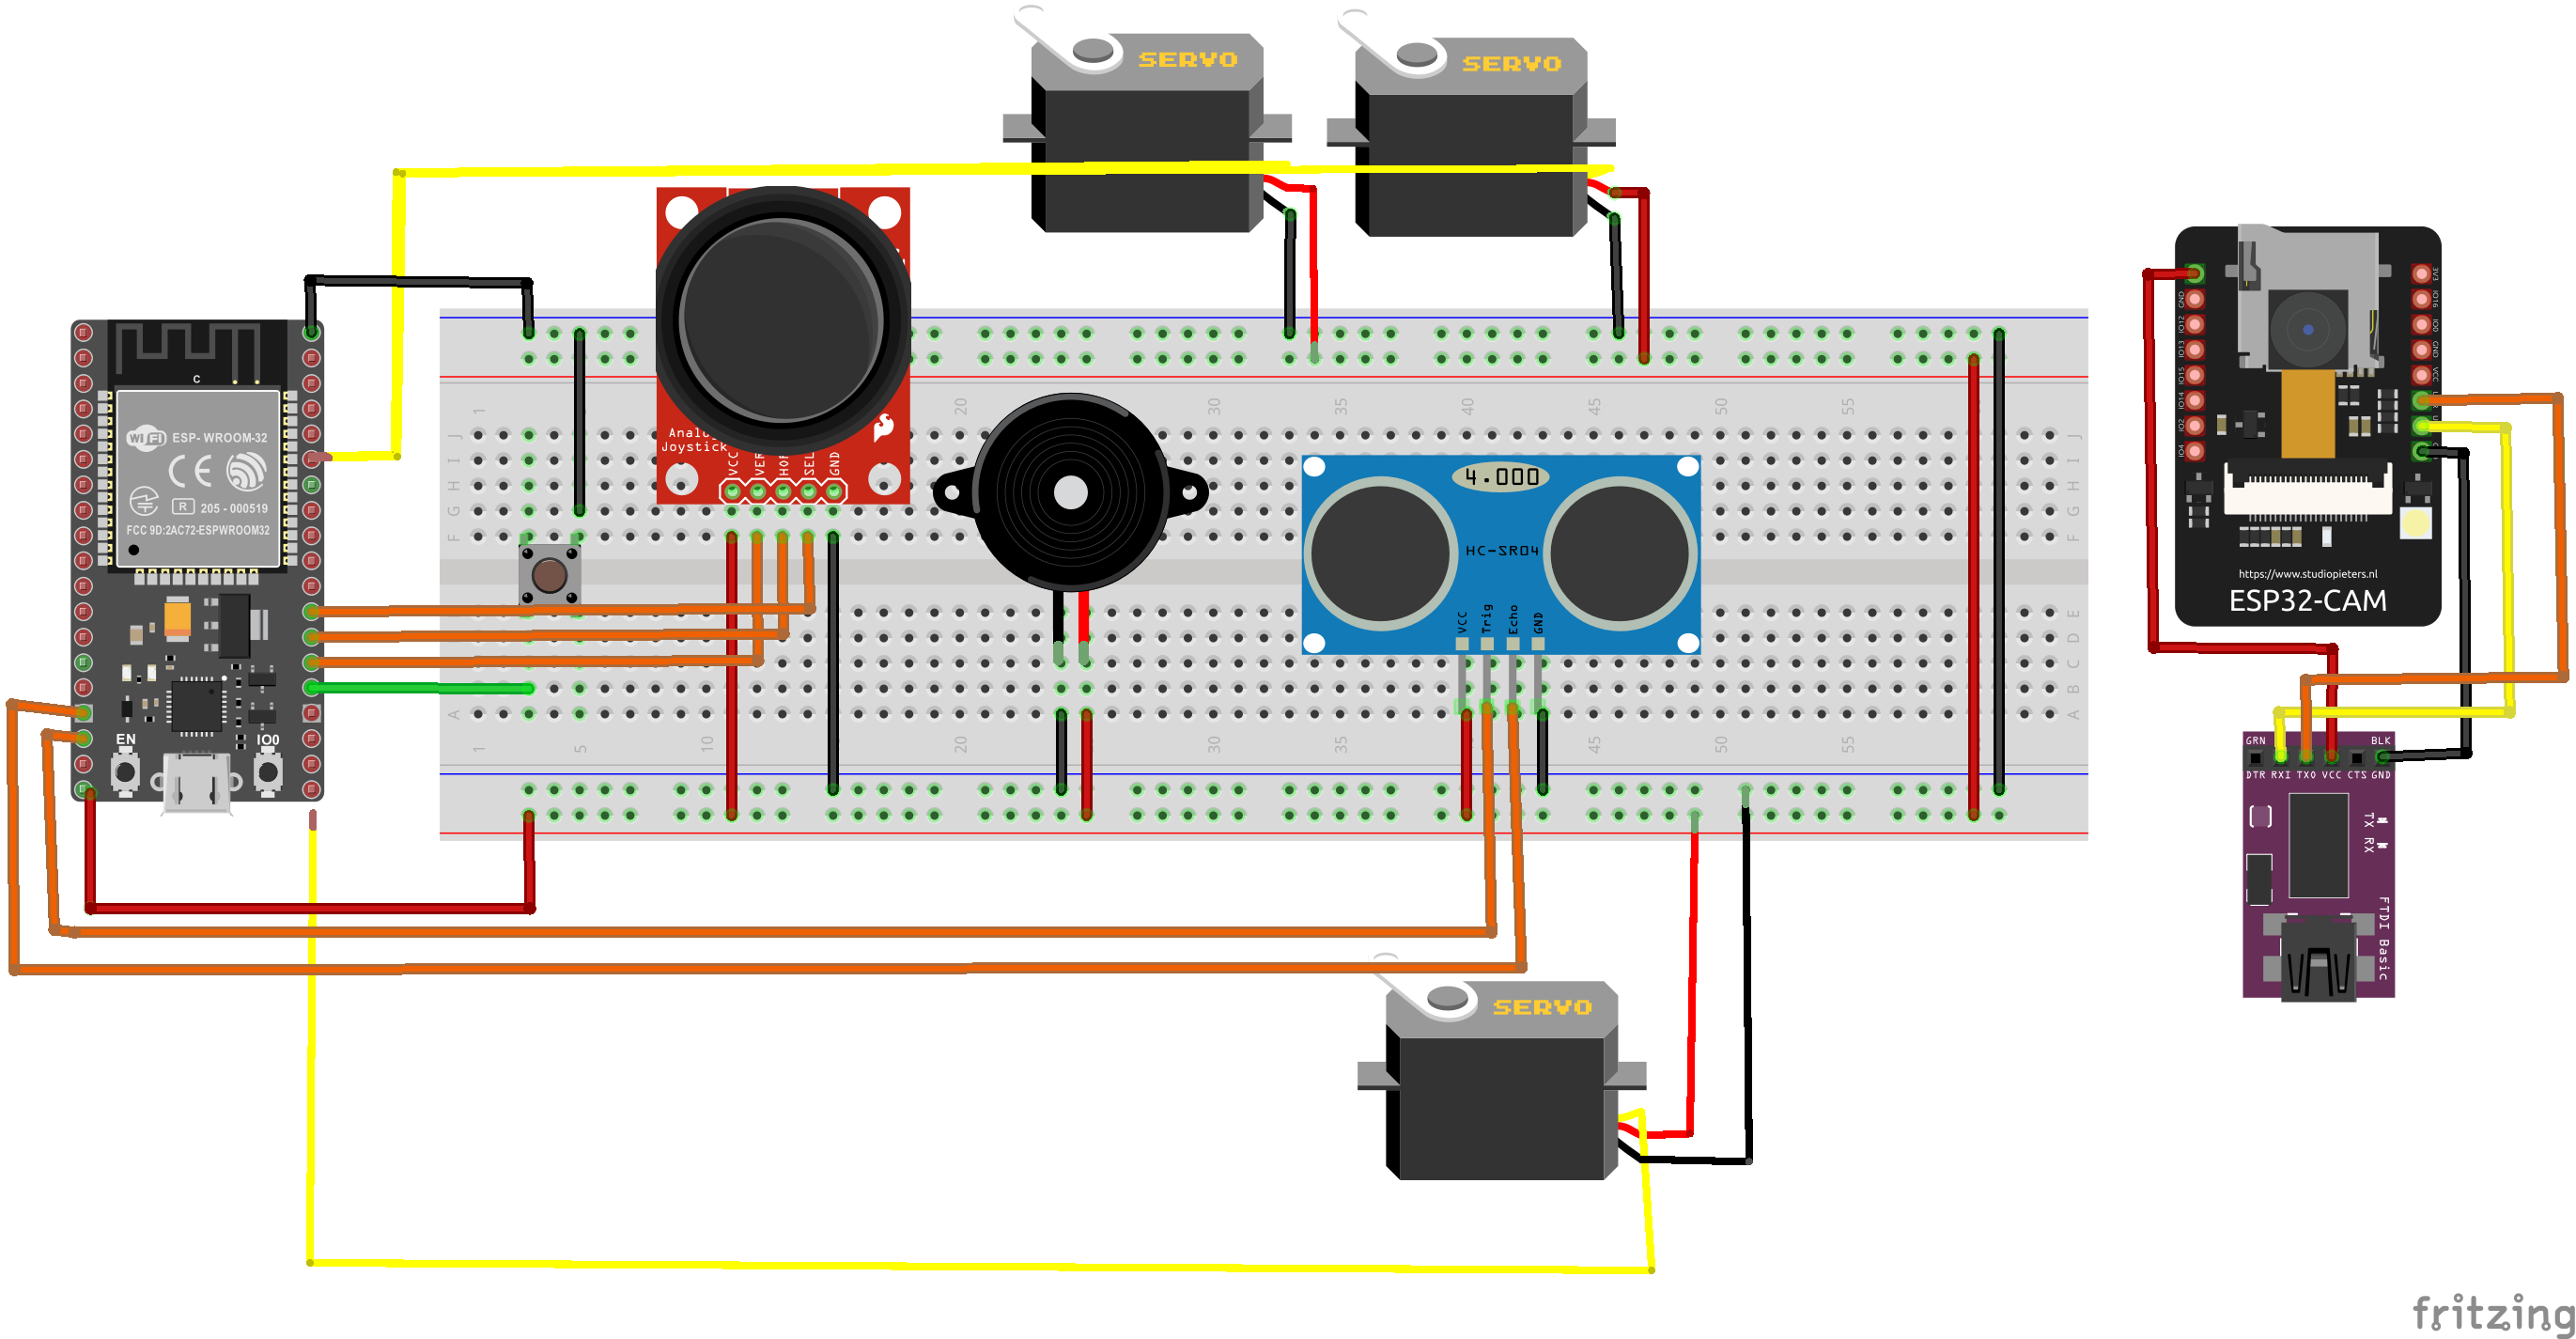
\includegraphics[width=8cm, height=4cm]{Lampiran/dig1.png}}
\caption{Wiring Diagram}
\label{dig}
\end{figure}

%BAB 4
\section{Code Structure}
In this final project, there are 2 codes used, namely the code for ESP32-Dev-Module and the code for ESP32-CAM.

\subsection{ESP32-Dev-Module}
The code for the ESP32-Dev-Module has a structure similar to the standard Arduino code, such as:
\begin{itemize}
\item At the beginning of the code, there is a line that states the use of the servo.h library. Then proceed with pin initialization for all hardware (except ESP32-CAM) as well as variables needed for the device to be made.
\item Continue on void setup() which contains the initialization of the pin mode used for each pin that was initialized previously. In this chart there is also the use of the Servo.h library in the form of initializing the pin number and the initial setting of the servo2 angle of 170°
\item In the void loop() there is a program that will run on the ESP32-Dev-Module. In this section, there is a statButton variable that reads the status of the push button which is the 'if' parameter. Branching is used because the tool can move 180° or can use a joystick. In this part of the void loop, we only need to call the ultrasonic sensor function if the push button is not pressed and call the joystick function if the push button is pressed.
\item void ultrasonik() is the function we created to run the ultrasonic sensor HC-SR04. As usual in this section there is a digitalWrite for trig and echo until finally getting the time value. The time value will be calculated according to the formula so that the object distance is obtained in CM units and the results will be written on the monitor.
\item void joystick() is the function used to run the joystick. in this function, there is a variable to store the input results from the joystick, and then it will be processed in a number range up to 180° with the map function. The results of the processing will be the angle of movement of the servo motor, be it servo1 or servo2.
\end{itemize}

\subsection{ESP32-CAM}
The code for the ESP32-CAM has a structure like AI-Thinker-Camera but in one files and the js for use COCO-SSD. All codes are property of ChungYi Fu (Kaohsiung, Taiwan).
\begin{itemize}
\item At the beginning of the code, there is a line that states the use of all library used. Then proceed with pin initialization for ESP32-CAM as well as variables needed for the device to be made like SSID and password for WiFi.
\item in void setup(), there is an initialization of a baud rate of 115200 and a configuration of all ESP32-CAM pins. In this section, the ESP32-CAM starts connecting to WiFi according to the specified SSID and password.
\item Furthermore, there is static which contains commands ranging from Capture Image screenshots, Video streaming, Command parameter control, Display video status parameters (must return json format to load initial settings), and Customize the homepage.
\item In static to Customize the homepage there is a line of HTML code that contains CSS, HTML body, and javascript. It is in this part of the javascript that the COCO-SSD model is called to classify objects captured by the ESP32-CAM.
\end{itemize}

%BAB 5
\section{Implementation Results}
Here we attach some of the results of the implementation of the tools we made in this final project. Some of these views are examples of demos that have been done to see the tools in use.

\begin{figure}[htbp]
\centerline{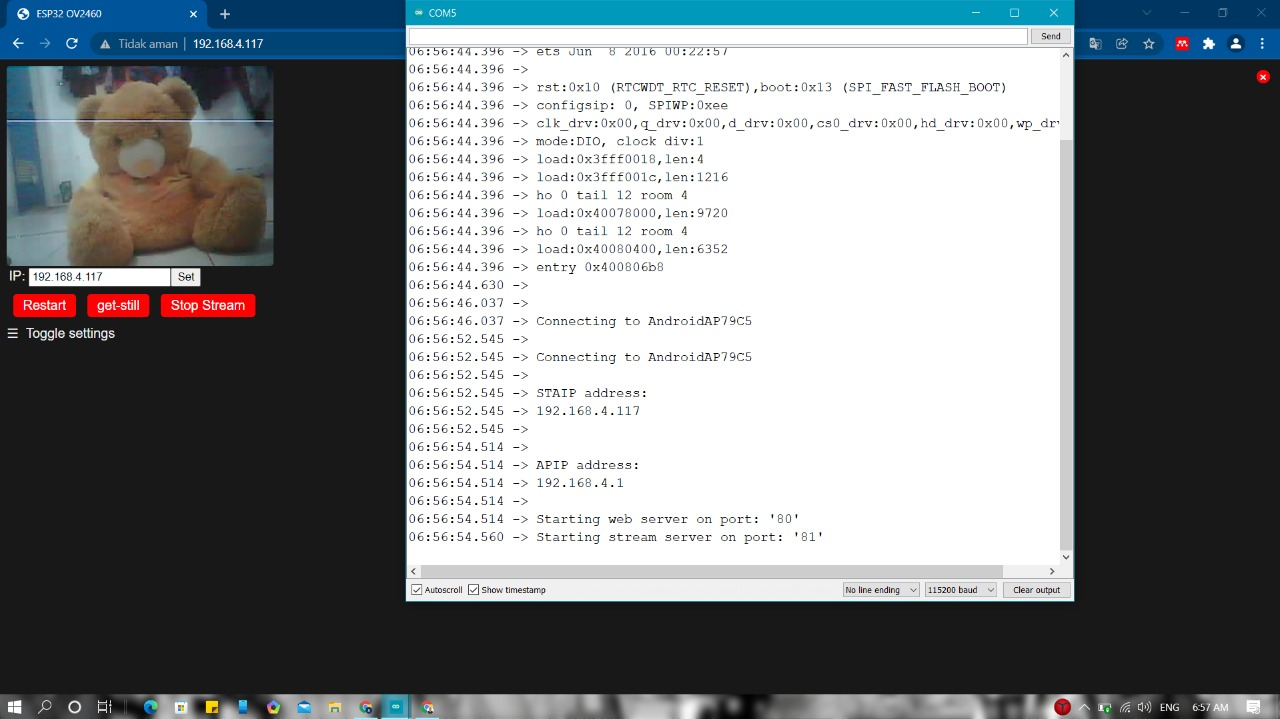
\includegraphics[width=8cm, height=4cm]{Lampiran/lam3.jpg}}
\caption{The ESP32-CAM performs the function to connect the ESP32-CAM to WiFi and obtain its IP Address.}
\label{lam3}
\end{figure}
\begin{figure}[htbp]
\centerline{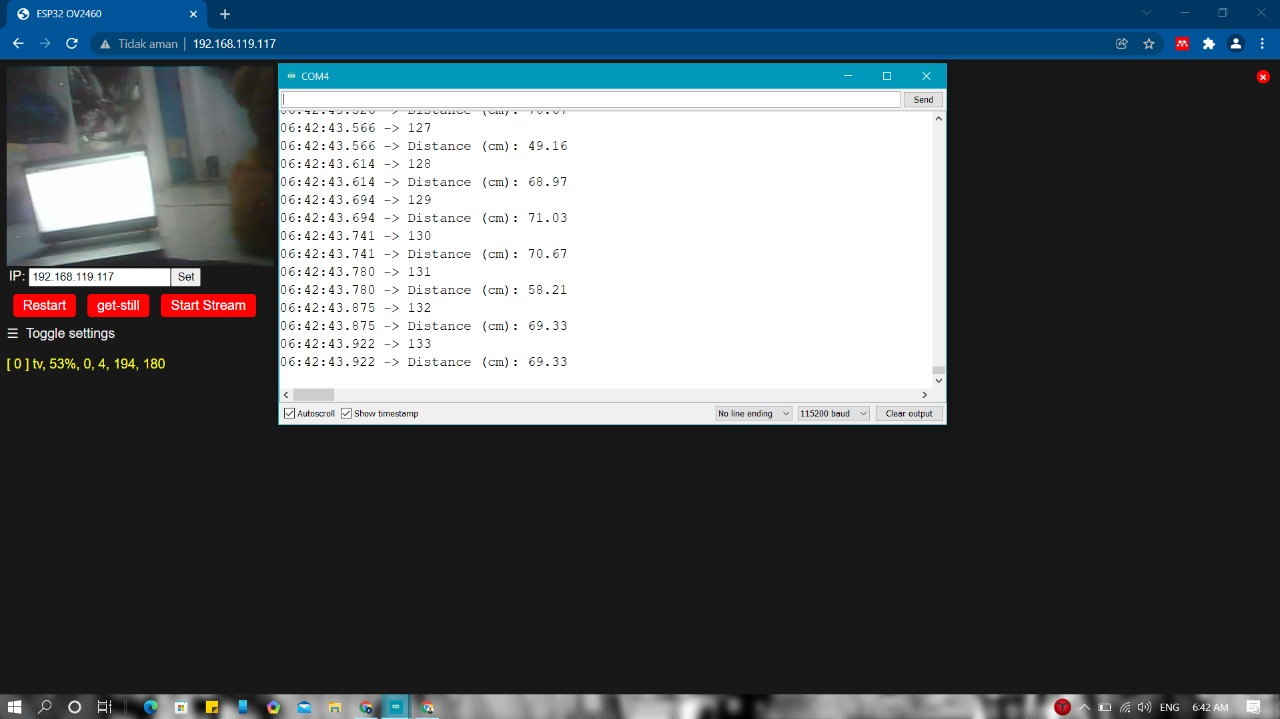
\includegraphics[width=8cm, height=4cm]{Lampiran/lam1.jpg}}
\caption{The movement of the servo motor can be seen on the monitor according to the specified baud rate. Then the results of the HC-SR04 ultrasonic sensor readings are also displayed}
\label{lam1}
\end{figure}
\begin{figure}[htbp]
\centerline{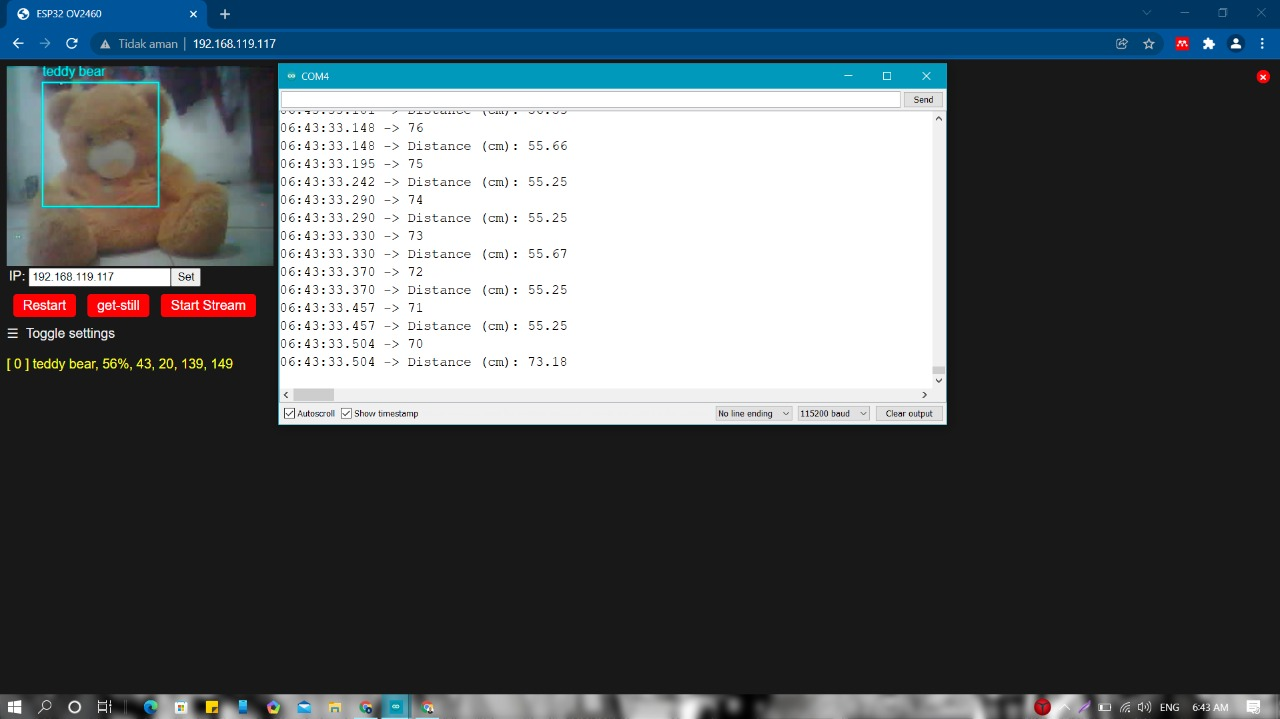
\includegraphics[width=8cm, height=4cm]{Lampiran/lam2.jpg}}
\caption{COCO-SSD provides object classification results by marking the object in question and calculating object size.}
\label{lam2}
\end{figure}
\begin{figure}[htbp]
\centerline{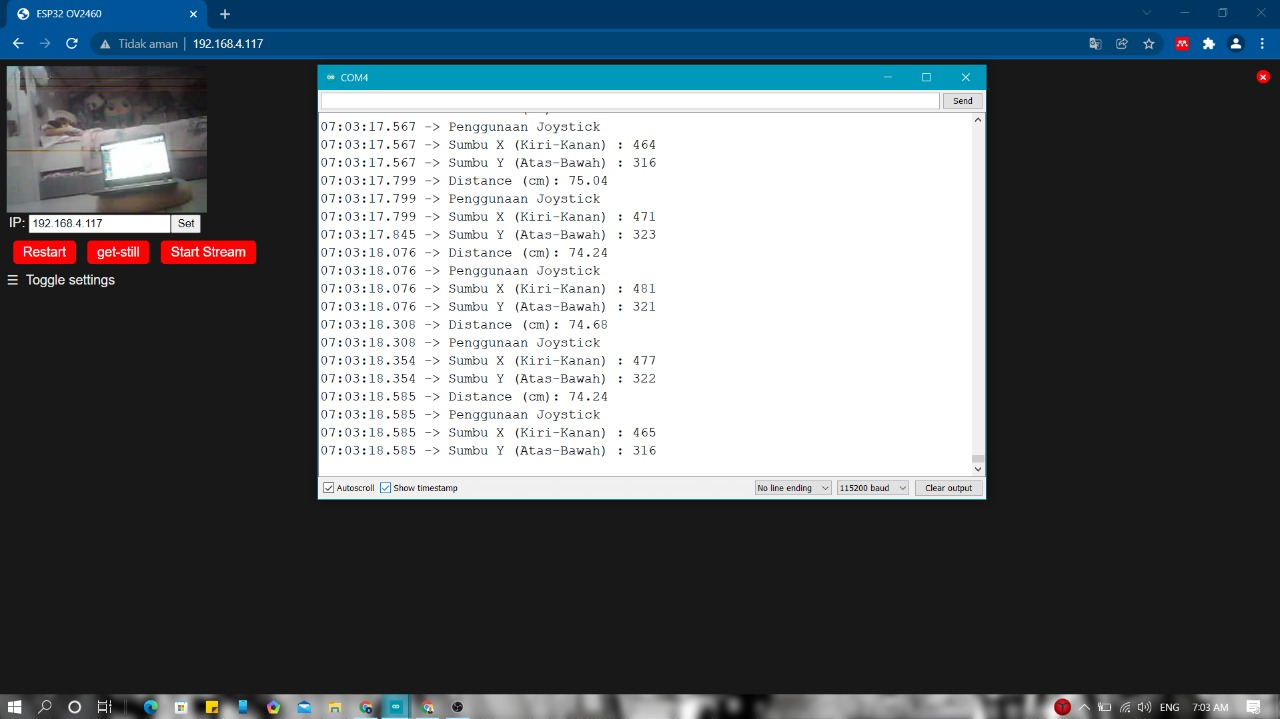
\includegraphics[width=8cm, height=4cm]{Lampiran/lam4.jpg}}
\caption{If use of the joystick will display the ultrasonic sensor readings as well and the joystick value.}
\label{lam4}
\end{figure}
\newpage
\begin{thebibliography}{00}
\bibitem{b1} L. RENALDI, S. HADIYOSO, and D. N. RAMADAN, “Purwarupa Radar sebagai Pendeteksi Benda Diam menggunakan Ultrasonik,” ELKOMIKA J. Tek. Energi Elektr. Tek. Telekomun. Tek. Elektron., vol. 6, no. 3, p. 317, 2018, doi: 10.26760/elkomika.v6i3.317.
\bibitem{b2} “Perbedaan Antara Radar dan Sonar”. [Online]. Available: https://id.sawakinome.com/articles/science--nature/difference-between-radar-and-sonar-2.html. [Accessed: 28-Oct-2021].
\bibitem{b3} Radar Ultrasonic | Sistem Mikroprosesor. (n.d.). Retrieved October 27, 2021, from https://sismik.stei.itb.ac.id/2017/05/23/radar-ultrasonic/
\bibitem{b4} Djuandi, Feri, 2011.“Pengenalan Arduino". Jakarta: Penerbit Elex Media. [Online]. Available : https://docplayer.info/30348975-Pengenalan-arduino-juli-2011-tingkat-oleh-feri-djuandi-pemula-menengah-mahir.html [Accessed: 29-Okt-2021]
\bibitem{b5} Liu, W., Anguelov, D., Erhan, D., Szegedy, C., Reed, S., Fu, C. and Berg, A., 2015. SSD: Single Shot MultiBox Detector.
\bibitem{b6} Saptaji, Handayani W. 2015. Mudah Belajar Mikrokontroller dengan Arduino. Bandung :Widya Media. [Online]. Available: https://doi.org/10.33096/ilkom.v9i3.158.282-289 [Accessed: 29-Okt-2021]
\bibitem{b7} Wicaksono, M. and Rahmatya, M., 2020. Implementasi Arduino dan ESP32 CAM untuk Smart Home. Jurnal Teknologi dan Informasi, 10(1), pp.40-51.
\end{thebibliography}
\end{document}
